\documentclass{beamer}
\usetheme[pageofpages=of,% String used between the current page and the
                         % total page count.
          bullet=circle,% Use circles instead of squares for bullets.
          titleline=true,% Show a line below the frame title.
          alternativetitlepage=true,% Use the fancy title page.
          titlepagelogo=images/logo-circl.pdf,% Logo for the first page.
%          watermark=watermark-polito,% Watermark used in every page.
%          watermarkheight=100px,% Height of the watermark.
%          watermarkheightmult=4,% The watermark image is 4 times bigger
                                % than watermarkheight.
          ]{Torino}


\usepackage[utf8]{inputenc}
\usepackage{tikz}
\usetikzlibrary{positioning}
\usetikzlibrary{shapes,arrows}
%\renewcommand\thefootnote{\hbox to 6pt{\hss\arabic{footnote}}}

\author{Alexandre Dulaunoy\emph{TLP:WHITE}}
\title{ENFORCE project - cybercrime training}
\subtitle{Improving the design of curriculum with practical information sharing}
\institute{}
%\date{\today}
\date{FIC 2020}


\begin{document}
% DO NOT COMPILE THIS FILE DIRECTLY!
% This is included by the other .tex files.

\begin{frame}[t,plain]
\titlepage
\end{frame}

\begin{frame}
        \frametitle{Curriculum developed}
\begin{itemize}
\item E.100 MISP - Open Source {\bf Threat Intelligence Platform Supporting Digital Forensic} and Incident Response
\item E.200 Post Mortem Analysis Techniques of Fake Invoices Manipulated PDF documents
\item E.201 {\bf Digital Forensics} - An introduction into Post-mortem Digital Forensics
\item E.202 {\bf Network forensic} - Analysing black-hole monitoring dataset - How to better understand DDoS attacks from backscatter traffic, opportunistic network scanning and exploitation
\item E.300 {\bf Data mining} using AIL framework
\item E.301 {\bf Cryptography Workarounds} For Law Enforcement
\end{itemize}
\end{frame}

\begin{frame}
        \frametitle{Development process}
        \begin{itemize}
                \item The development process is to bring together {\bf forensic analysis, information sharing and information exchange}.
                \item The {\bf law enforcement contribution is critical and helps us to improve open source software} such as MISP and the training materials at large for the LE community.
                \item {\bf The sessions are interactive} and we work together on solving cases, discovering new findings and techniques on a real environment running on a Cyber Range platform (HNS).
        \end{itemize}
\end{frame}

\begin{frame}
        \frametitle{Training setup to support information sharing}
        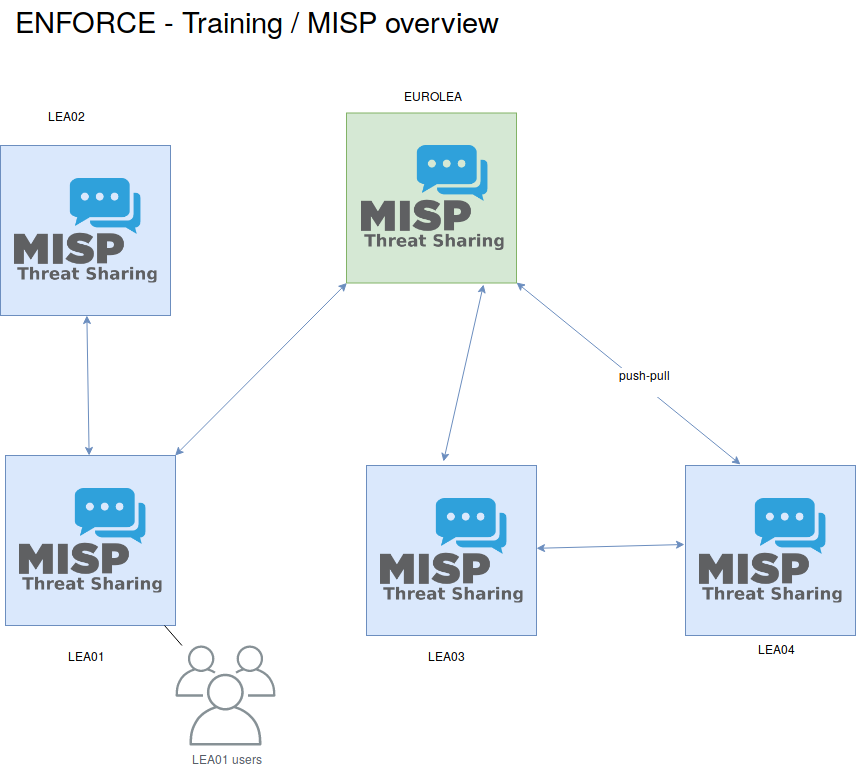
\includegraphics[scale=0.27]{enforce-misp.png}
\end{frame}


\begin{frame}
\frametitle{Practical outcomes of the ENFORCE project}
        \begin{itemize}
                \item {\bf Direct improvements into open source software} used by law enforcement
                \item The complete ENFORCE curriculum {\bf will be open sourced} in May 2020
                \item {\bf Ensuring the sustainability of the project} via contributors in various fields such as law enforcement
        \end{itemize}
\end{frame}



\begin{frame}
\begin{itemize}
\item Contact: info@circl.lu
\item \url{https://www.circl.lu/}
\item \url{https://www.misp-project.org/}
\item \url{https://github.com/MISP} - \url{https://twitter.com/MISPProject}
\item Don't hesitate to get in touch with us to access one of our sharing community or feedback to improve MISP.
\end{itemize}

\end{frame}

\end{document}

